% TEMPLATE for Usenix papers, specifically to meet requirements of
%  USENIX '05
% originally a template for producing IEEE-format articles using LaTeX.
%   written by Matthew Ward, CS Department, Worcester Polytechnic Institute.
% adapted by David Beazley for his excellent SWIG paper in Proceedings,
%   Tcl 96
% turned into a smartass generic template by De Clarke, with thanks to
%   both the above pioneers
% use at your own risk.  Complaints to /dev/null.
% make it two column with no page numbering, default is 10 point

% Munged by Fred Douglis <douglis@research.att.com> 10/97 to separate
% the .sty file from the LaTeX source template, so that people can
% more easily include the .sty file into an existing document.  Also
% changed to more closely follow the style guidelines as represented
% by the Word sample file. 
% This version uses the latex2e styles, not the very ancient 2.09 stuff.
\documentclass[twocolumn, 10pt]{article} 
\setlength{\columnsep}{0.15in}
\usepackage{graphicx,fullpage,epsf,epsfig,endnotes,url}
\usepackage[T1]{fontenc}
\usepackage{pslatex}
\usepackage{times}
\begin{document}

% replace the name to unblind
\newcommand{\DataSeries}{DataSeries}
\newcommand{\DS}{DS}
%\date{}

%make title bold and 14 pt font (Latex default is non-bold, 16 pt)
\title{\Large \bf \DataSeries{}: An efficient, flexible data format for structured serial data}

\author{
\begin{tabular}{c}
DataSeries Technical Documentation \\
software@cello.hpl.hp.com \\
\end{tabular}
}

% TODO: figure out how/where to put this into the documentation

% Major authors: 
%    Eric Anderson <eric.anderson4@hp.com>
%    Martin Arlitt <martin.arlitt@hp.com>
%    Charles B. Morrey III <brad.morrey@hp.com>
%    Alistair Veitch <alistair.veitch@hp.com>

\maketitle

% Use the following at camera-ready time to suppress page numbers.
% Comment it out when you first submit the paper for review.
%\thispagestyle{empty}

{ \Large Note: some of the experiments described are
  based on old versions of the DataSeries code, prior to many of the
  later improvements.  This tr snapshot built from the 2008-02-27
  version of the source with this note added.  }
\subsection*{Abstract}
We describe methods to capture, convert, store and analyze NFS
workloads that are 20-100$\times$ more intense, in terms of
operations/day, than any previously published.
%
We describe three techniques that improve capture performance by up to
$10\times$ over previous techniques.
%
For conversion, we use a general-purpose format that is both highly
space efficient and provides efficient access to the trace data.
%
For
analysis, we describe a number of techniques adopted from the
database community and some new techniques that facilitate analysis of 
very large traces.
%
We also describe a number of guidelines for trace collection that should
prove useful to future practitioners.
%
Finally, we analyze a commercial feature
animation (movie) rendering workload using these techniques and discuss the
characteristics of the workload.
%
Our implementation of these techniques is available as open source
and the exact anonymized datasets we analyze are available for free download.

% LocalWords:  anonymized


\section{Introduction}

\fix{11. Another word rather than intense in title?}
\fix{13. More motivation on why we do tracing -- if we can get the space}
Storage tracing and analysis has a long history.  Some of the earliest
filesystem traces were captured in 1985~\cite{ousterhout85}, and there
has been intermittent tracing effort since then, summarized by
Leung~\cite{LeungUsenix08}.  These traces are
analyzed to find properties that future systems should support or
exploit, and as input to simulators and replay tools to explore system
performance with real workloads.

One of the problems
with trace analysis is that old traces inherently have to be scaled up
to be used for evaluating newer storage systems because the
underlying performance of the newer systems has increased.  Therefore,
the community benefits from regularly capturing new traces from multiple
sources, and if possible, traces that put a heavy load on the storage
system, reducing the need to scale the workload.

Most traces, since they are performed by academics, are captured in
academic settings.  This means that the workloads captured are
somewhat comparable, but it also means that commercial workloads are
under-emphasized.  Microsoft is working to correct this by capturing
commercial enterprise traces from their internal
servers~\cite{snia-iotta-microsoft}.  Our work focuses on commercial
NFS~\cite{rfc1094nfs} workloads, in particular from a feature animation (movie) company.
The name of the company remains blinded as part of the agreement to
publish the traces.  The last publically available NFS traces that we
are aware of were collected in 2003.  Our 2003 and 2007
traces~\cite{animation-bear-traces} provide recent NFS traces for use
by the community.

One difference between our traces and other ones is the data rates
that we measured.  Our 2003 client traces saw about 750 million
operations per day.  In comparison, the 2003 Ellard
traces~\cite{EllardLisa03} saw a peak of about 125 million NFS
operations per day, and the 2007 Leung traces~\cite{LeungUsenix08}
saw a peak of 19 million CIFS operations/day.  Our 2007 traces saw
about 2.4 billion operations/day.  This difference required us to
develop and adopt new techniques to capture, convert, and analyze the
traces.

Since our traces were captured in such a different environment than
prior traces, we limit our comparisons to their workloads, and we
do not attempt to make any claims about trends.  We believe that
unless we, as a community, collect traces from hundreds of different
sites, we will not have sufficient data to make claims stronger than
``this workload is different from other ones in these ways.''  In
fact, we make limited comparison in the trends between our 2003 and
2007 traces for similar reasons.  The underlying workload changed
as the rendering techniques improved to generate higher quality output,
the operating system generating the requests changed, the NFS
protocol version changed, and the configuration of the clients 
changed because of standard technology trends.

The process of understanding a workload involves four main
steps, as shown in Figure~\ref{fig:overall-process}.  Our tools for
these steps are shown in italics for each step, as well as some
traditional tools.  The first step is capturing the workload, usually
as some type of trace.  The second step is conversion, ususally from
some raw format into a format designed for analysis.  The third step
is analysis to reduce the huge amount of converted data to
something manageable.  Alternately, this step is a simulation or replay to
explore some new system architecture.  Finally the fourth step is to
generate graphs or textual reports from the output of the analysis or
simulation.

Our work has five main contributions:

\begin{enumerate}
\item The development of techniques for lossless raw packet capture up to
5Gb/s, and with the hardware improvements since our work, likely to
10Gb/s.  These techniques are applicable to anyone wanting to capture
a network storage service such as NFS, CIFS, or iSCSI.

\item A series of guidelines for the conversion and storage of the
traces.  Many of these guidelines are things that we wish we had known
when we were converting our traces.  We used
DataSeries~\cite{DataSeriesOSR2009} to store the traces, but our
guidelines are general.

\item Improved techniques for analyzing very large traces that allow
us to look at the burstiness in workloads, and an examination of how
the long averaging intervals in prior analysis can obscure workload
properties.

\item The analysis of an intense NFS workload demonstrating that our
techniques are successful.

\item The agreement with the animation company to allow the roughly
100 billion operation anonymized traces to be published, along with
the complete set of tools to perform all the analysis presented in
this paper and to generate the graphs.  Other
researchers can build on our tools for further analysis, and use
the traces in simulation studies.
\end{enumerate}

\begin{figure}
\center 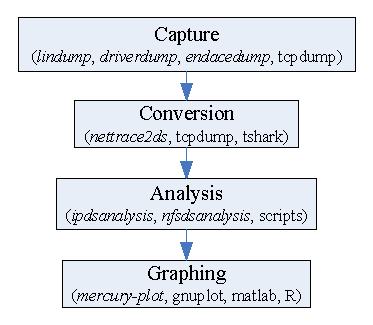
\epsfig{width=2.2in, angle=0, file=overall-process.eps}
\caption{Overall process; our tools are shown in italics, traditional tools
after them.}
\label{fig:overall-process}
\end{figure}

We examine related work in section~\ref{sec:related}.  We describe our
capture techniques in section~\ref{sec:capture}, followed by the
conversion (section~\ref{sec:conversion}). We describe our adopted and
new analysis techniques in section~\ref{sec:analysis-techniques} and
use them to analyze the workload in section~\ref{sec:analysis}.
Finally we conclude in section~\ref{sec:conclusion}.

\section{Related work}

related work goes here


\section{Design}\label{sec:design}

DataSeries is intended to provide streaming access to structured serial
data. Corresponding
to the first four properties\footnote{The fifth property, an expressive
programming interface, is described in Section~\ref{sec:programming}.}
described in the introduction, DataSeries was designed with the
following goals in mind. First, it should be very storage
efficient. Second, it must be efficient to encode, decode and
interpret the data.  Third, the format should not constrain the
types of information to be stored. Fourth, the internal data must be
self-describing, i.e., the names and types of the data stored have to
be determined by the contents of the file itself, rather than 
externally.

\subsection{File structure}\label{sec:structure}

\begin{figure*}
% \vspace{-0.6cm}
\hfil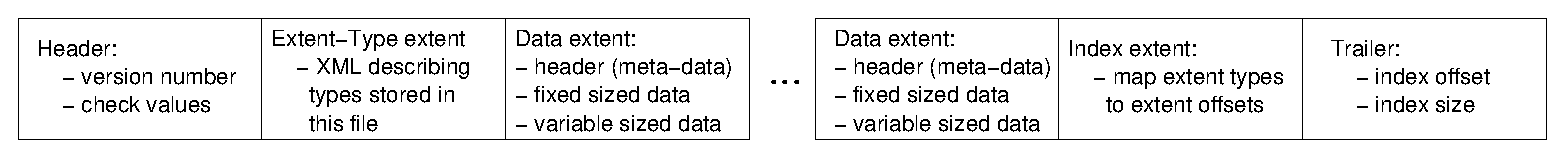
\includegraphics[width=6.5in]{fig/ds-format2.eps}\hfil
\caption{Internal structure of a DataSeries file. }
\label{fig:dsorg}
% \vspace{-2mm}
\end{figure*}

DataSeries' data model is conceptually very similar to that used
by relational databases. 
Logically, a DataSeries file is composed of an ordered sequence of
{\it records}, where each record is composed from a set of {\it
fields}. Each field has a {\it field-type} (e.g., integer, string, double,
boolean) and a name. A DataSeries record is analogous to a row in a
conventional relational database. We call the type of a row 
the {\it extent-type} because 
an {\it extent} contains a collection of rows with the same fields and 
field-types.

A single DataSeries file comprises a
collection of extents (potentially with different extent-types), plus a
header and extent-type extent at the beginning of the file, and an index extent and
trailer at the end of the file. Figure~\ref{fig:dsorg} shows
this organization.  The extent-type and index extents are the same as the
other extents in the file except that their names and extent-types are 
hard-coded in the library.

The header on a DataSeries file contains the DataSeries file version,
and five check values 
to determine the encoding format for integers and doubles.
DataSeries files
are always written out using the native formats of the system doing
the writing. We did this to minimize byte-swapping overheads,
as usually the architecture reading the files is the same 
as the architecture writing the files.
The library transparently does endianness conversions in the 
rare circumstances that this is not true, and also provides a ``repack''
utility for explicit conversion.

Immediately following the header is the extent-type extent. Records in
this extent have a single string-valued field, each of which 
contains an XML specification that defines the extent-types of all the 
other extents in the file.  

% TODO: get the xml figure example working again.

% Figure~\ref{fig:xml} shows an example of the XML used to describe an extent-type.
% \begin{figure}
%  \vspace{-0.6cm}
% \hfil
% \includegraphics[width=2.8in]{fig/xml.eps}
% \hfil
% \caption{Example XML used to describe extent types, as described in
% Section~\ref{sec:structure}. Section~\ref{sec:extenttype} discusses
% extent typing while Section~\ref{sec:options} describes the opt\_* and
% pack\_* options. }
% \label{fig:xml}
% % \vspace{-2mm}
% \end{figure}

When reading a DataSeries file, the trailer is read next.  It consists
of the offset and size (after compression) of the index extent.  The
offset is used to read the index extent, which has two fields, an
extent-type and an offset, to allow direct access to extents of a single type.
The index and trailer are
stored in this order, at the end of the file, to enable efficient
writing. The writer will often not know, a priori, what the final
extent sizes will be, so space for the index cannot be allocated until
after the extents have been written.

The data extents themselves consist of a header, followed by the 
fixed size data
and the variable sized data.  Both fixed and variable sized data may be
compressed, using any one of a number of standard compression
algorithms~\cite{GZIP,BZIP,LZF,LZO}.  The header contains metadata
about the data in the extent, such as the compressed sizes of the
fixed and variable data, the number of records in the extent, the
uncompressed size of the variable length data, the compression mode,
the extent-type of the extent, and checksums of the extent before and
after compression to guard against hardware and software errors.
Checksum validation can be disabled during extent reading to improve
performance at the cost of reduced reliability.

Each row in the fixed size data is stored as a structure, with the fields sorted by size and with 
padding between sizes.
In particular, in each row, all of the boolean fields are packed, then all
the byte fields, padding is added to align to a 4 byte boundary, and
then the 4 byte integer and variable offset pointers are packed.
Lastly, the structure is padded to an 8 byte boundary and the 8 byte
integer and double fields are packed. When uncompressed, this layout
allows for very efficient access to data: every field can be accessed
through a pointer to the row, using a single addition and deference. 
This access method achieves goal two -- efficient decoding and
interpretation of the data.

\subsection{Extent types and options}\label{sec:extenttype}

An extent-type in DataSeries defines the field-type of all the fields in a
related group of records.  Every extent-type has a name; this is
intended to be a general description of the record.  We have found that
using a naming convention that encodes type and hierarchical information,
such as 
Trace::BlockIO::HPUX, 
Trace::NFS::common or
Trace::NFS::read-write
%, or 
%\linebreak[4] Summary::Network::IP::bandwidth-rolling
works well, providing information to the user on what is contained, and 
about extents that may be related (e.g., the Trace::NFS::* names above). 
% NFS::common and
% \linebreak[4] NFS::read-write). 
The extent-type also has a namespace to avoid naming conflicts between
organizations and a version number to make it easy to test whether
a program is compatible with a particular extent-type.
% We previously used a format with spaces in it, but
% found this was inconvenient to use with command line tools.  
% INCLUDE IN EXTENDED VERSION
%% To handle
%% the case where different organizations happen to use the same
%% name, each extent type also has a namespace which is intended to be a
%% domain or host name and has the semantics that two people who
%% independently choose names will choose different namespaces.  
%% Finally,

% Update ExtentType.hpp if you change this.

The extent type also has a version number of the form major.minor with the
semantics that minor versions are only allowed to add new fields,
whereas major versions can remove fields, rename fields or change
field semantics.  This means that analysis code that can process
version 1.x will work on any version 1.y for y $\geq$ x, but may or may not
work on version 2.0.

\subsection{Data types}

DataSeries currently supports six data types:
\textbf{bool} (0 or 1),
\textbf{byte} (0-255),
\textbf{int32} (signed 32bit integer),
\textbf{int64} (signed 64bit integer),
\textbf{ double} (IEEE 64 bit floating point), and
\textbf{variable32} (up to $2^{31}$ bytes\footnote{This could be changed to $2^{32}$ bytes by use of unsigned instead of signed.} of variable length data, such as strings).
% This is typically used for recording string values.

Supporting additional data types is a straightforward extension that
does not require changing the version of DataSeries.  In practice we
have found these data types to be sufficient.
% for the many types of data we have stored.  
%Section~\ref{sec:lessons} discusses some possible extensions.

\subsection{Options}\label{sec:options}

In addition to the types that are supported, there are a number of
options that can be applied to the data types.  Options are either of
the form opt\_*, or pack\_*; the former extend or change the values
available to applications, and require applications to understand the
option, whereas the latter form are transparent to applications, but
enable higher compression than would otherwise be available. Options
are applied to either an entire extent or to individual fields.  One
possible direction for future work would be automatically inferring
the ``best'' packing options.

\subsubsection{Extent-level options}

Extent level options control the way the entire extent is stored.
Currently there are three options here:

\begin{enumerate}

\item pack\_null\_compact: Should we remove all of the nullable fields
before running the results through compression.  For records with many
nullable values this can greatly increase the compression ratio at a
cost of additional computation time.  See section~\ref{sec:ellard} for
an evaluation of this option.

\item pack\_pad\_record: This option controls how the record is
padded.  Originally all records were padded to 8 bytes.  For records
with only 4 byte or smaller fields, this wastes some amount of space,
and hence the option to pad to the maximum column size was added.  See
section~\ref{sec:world-cup-1998} for an evaluation of this option.

\item pack\_field\_ordering: This option controls how the fields are
ordered within a record.  It turns out some files compress better with
different field orderings.  See section~\ref{sec:world-cup-1998} for
an evaluation of this option.

\end{enumerate}

\subsection{Field-level Options}

Field-level options control the meaning of individual fields (for
opt\_* options), or how that field is represented before compression
(for pack\_* options).  Options include:

\begin{enumerate}

\item opt\_nullable: Indicates values in this column can be null.
This option is
implemented by generating a hidden boolean column that determines if
the value is null.

\item opt\_doublebase={\it base-value}: Specifies a relative base for
doubles.  This is used to gain additional precision in the double
without losing the absolute value.  
This is particularly useful for storing Unix time stamps with nanosecond
precision.
%In particular, we have found this
%useful for storing time in seconds in Unix time\footnote{Unix time has an epoch
%start of 12AM, 1 January 1970.}, but with a precision in nanoseconds, which
%would otherwise be impossible as an IEEE double has insufficient
%precision.

\item pack\_scale={\it scale-value}: This specifies the precision to use for
double values.
% INCLUDE IN EXTENDED VERSION
%; in particular it means that the double will be
%multiplied by 1/{\it scale-value}, and rounded to an integer before
%being compressed, with the reverse transform applied after the data is
%uncompressed.  This option is useful because values that are stored as
%doubles sometimes accumulate pseudo-random bits in the low
%digits.  These pseudo-random bits contain no useful information and
%reduce the achievable compression.
This option improves compression by removing the pseudo-random bits in the low 
bits of doubles by scaling and rounding the double.  

\item pack\_relative={\it field-name}: Specifies that this field
should be packed relative to another field.  This delta encoding
option is useful for compressing time stamps and other values which
may be large but are usually close to the previous value in the same
field or the value of a different field in the same row.  In
particular it means that if {\it field-name} is the same as the
current field's name, the previous row's value will be subtracted from
the current row's value before the data is compressed, and otherwise
from the value of the other field in the same row.  This feature is
only supported for int32, int64, and double fields.  For double fields
it is required that the fields be packed with pack\_scale as well to
eliminate precision issues.

\item pack\_unique: Specifies that each unique variable32 value
should only be packed once within that extent.  This option applies across all variable32
fields with pack\_unique enabled.  For fields with many repeated
values this option can significantly increase the effective
compression ratio because it entirely removes duplicate data within that extent
(compression algorithms only remove it partially).

\end{enumerate}

\subsection{Design summary}

The DataSeries file format was designed to allow for flexibility
(through the use of a self-contained and extensible type description
for extents) and performance (through extensive use of compression and
a data layout that allows for direct access to data values). 
Section~\ref{sec:results} describes experiments using
DataSeries that quantitatively validate these claims.


% TODO add something about time formats in here; include http://cr.yp.to/libtai/tai64.html
\section{File format specification}

This section provides a precise specification of the DataSeries
version 1 file format.  A conformant dataseries file must consist of
the following sections, as shown in figure~\ref{fig:dsorg}:

\begin{enumerate}
\item {\bf header}: The header includes the version number and check values.
\item {\bf extent-type extent}: The extent defining the types used in the file.
\item {\bf data extent}: Zero or more extents comprising data types defined in the extent-type extent.
\item {\bf index extent}: An extent indexing the types and locations of each exxtent.
\item {\bf trailer}: The trailer contains the offset of the index extent, and some additonal check values.
\end{enumerate}

A conformant implementation may parse files that are missing the index
or the trailer.  The extent-type extent and index extent are simply
data extents with pre-known types, and so will be described after we
specify the extent format.  A valid file must use the same byte
ordering for all values in a file.  A conformant implementation must
support both big endian and little endian orderings.

\subsection{types}

This specification defines the following types:

\begin{enumerate}
\item {\bf byte}: A one byte (8 bit), value ranging from 0..255
\item {\bf int32}: A four byte (32 bit) signed two's complement value stored in host-byte order.
\item {\bf int64}: An eight byte (64 bit) signed two's complement value stored in host-byte order.
\item {\bf double}: An eight byte (64 bit) IEEE 754 floating point value stored in host-byte order.
\end{enumerate}

\subsection{header}

The DataSeries header is used to validate that a file is being
properly parsed. A conformant implementation should validate the
contents of the header, e.g. by calling isnan on the NaN check value.
The header must consist of the following values:

\begin{enumerate}
\item {\bf file-type}: Four bytes, 'DSv1' in ASCII, 0x44, 0x53, 0x76, 0x31 in hexadecimal
\item {\bf int32 check value}: In file byte order, 0x12345678
  (big endian = 0x12, 0x34, 0x56, 0x78; little endian = 0x78, 0x56, 0x34, 0x12).
\item {\bf int64 check value}: In file byte order, 0x123456789ABCDEF0
  (big endian 0x12 0x34 0x56 0x78 0x9a 0xbc 0xde 0xf0; little endian =
  0xf0 0xde 0xbc 0x9a 0x78 0x56 0x34 0x12).
\item {\bf double check value}: The double constant
  3.1415926535897932384 in file byte order.  (big endian 40 09 21 fb
  54 44 2d 18; little endian 18 2d 44 54 fb 21 09 40)
\item {\bf infinity check value}: The double IEEE +$\infty$ floating
  point constant  (big endian 7f f0 00 00 00 00 00 00; little endian
  00 00 00 00 00 00 f0 7f).
\item {\bf NaN check value}: Any double IEEE NaN floating point
  constant in file byte order.
\end{enumerate}

\subsection{trailer}

The DataSeries trailer is used to locate the index extent.  A
conformant implementation should validate the trailer, but may choose
to tolerate an invalid trailer.  The trailer consists of the following
bytes:

\begin{enumerate}
  \item {\bf constant bytes}: Four bytes, 0xFF, 0xFF, 0xFF, 0xFF.
  \item {\bf index extent size}: int32 in file byte order, byte size of
    the index extent in the file.
  \item {\bf inverse extent size}: int32 in file byte order, bitwise
    complement of the index extent size.
  \item {\bf semi-random bytes}: int32 in file byte order, an arbitrary
    32 bit integer.  The implementation should chose this value derived
    from the extents in a file so that file contents are reproducable.
  \item {\bf index extent offset}: int64 in file byte order, offset in
    bytes from the beginning of the file for the index extent.
  \item {\bf hash bytes}: int32 in file byte order, bob-jenkins lookup-2
    hash~\cite{bob-jenkins-hash-lookup-2} of the above bytes. 
\end{enumerate}

\subsection{extent}

An extent in a dataseries file stores the actual data of a dataseries
file, or the two special extents in the file.  An extent consists of
the following bytes:

\begin{enumerate}

  \item {\bf compressed fixed-data size}: int32 in file byte order,
    byte size of the compressed representation of the fixed data.

  \item {\bf compressed variable-data size}: int32 in file byte order,
    byte size of the compressed representation of the variable data.

  \item {\bf number of records}: int32 in file byte order, count of
    the number of records (rows) in this extent.

  \item {\bf uncompressed variable-data size}: int32 in file byte order, 
    byte size of the variable representation after it has been uncompressed.
   TODO-eric: does this include the 4 0 bytes in the in-memory rep?

  \item {\bf compressed adler32 digest}: int32 in file byte order, 
    adler32 digest of the compressed data.
    TODO-eric: how calculated...

  \item {\bf partly-unpacked bob-jenkins hash}: int32 in file byte order,
    bob-jenkins hash of the data after it has been partly unpacked.
    TODO-eric: how calculated...

  \item {\bf fixed-records compression algorithm}: byte; index of the
    compression algorithm used for the fixed-data.  Valid compression algorithms
    are shown in section~\ref{sec:ff:compression-types}.

  \item {\bf variable-records compression algorithm}: byte; index of the
    compression algorithm used for the variable-data.  Valid compression algorithms
    are shown in section~\ref{sec:ff:compression-types}.

  \item {\bf extent type name length:} byte; length of the extent-type
    name.

  \item {\bf unused zero byte} byte; 0.  (pad to round up the header to multiple of 4 bytes)

  \item {\bf type name} {\it extent type name length} bytes.  Extent
    type name for the current extent.  Must be either one of the two
    pre-defined types, or one of the types defined in the extent-type
    extent.

  \item {\bf padding} 0--3 bytes; sufficient 0 bytes to pad the
    current offset to 4 byte alignment.  For example, if the type name
    is 7 bytes long, the padding would consist of 1 byte of 0.

  \item {\bf compressed fixed-data} {\it compressed fixed-data size}
    bytes.  The compressed bytes storing the fixed data.

  \item {\bf padding} 0--3 bytes; sufficient 0 bytes to pad the
    current offset to 4 byte alignment.  For example, if the
    compressed fixed-data size is 128, there would be no padding.

  \item {\bf compressed variable-data} {\it compressed variable-data size}
    bytes.  The compressed bytes storing the variable data.

  \item {\bf padding} 0--3 bytes; sufficient 0 bytes to pad the
    current offset to 4 byte alignment.  For example, if the
    compressed variable-data size is 9, the padding would consist of 3
    bytes of 0's.
\end{enumerate}

\subsection{Compression types}
\label{sec:ff:compression-types}

TODO-eric: fill-in



\section{Programming}\label{sec:programming}

Programming in dataseries is now described as part of the DataSeries User Guide
$<$https://github.com/dataseries/DataSeries/wiki/Dataseries-user-guide$>$.


\section{Performance Results}\label{sec:results}
We performed various experiments to measure the effectiveness of
\DataSeries{}' compression techniques, and then further compared other
types of data encoding and analysis tools for compression and
execution speed.  We first describe the experimental setup, then the
workloads, the benchmarks, and finally our results.

\subsection{Experimental setup}

The test-bed we used to perform most of the quantitative benchmarks for
this work was a cluster of 18 servers configured for batch processing of single server jobs.  Each server had one
or two dual core Opteron 280 2.4GHz processors.  Each processor had
64KB of L1 D-cache and 1024KB of L2 cache.  Additionally, each server
was configured with 4GB of main memory and could access a 10TB NFS
filesystem over 1Gb/s Ethernet, the underlying storage being RAID6 in
the form of HP MSA20 and MSA60 disk arrays.  The cluster was configured with
RedHat Enterprise Linux 4 and each server was running the 2.6.9 SMP
x86\_64 kernel version.  
% Results on a separate Xeon cluster showed
% similar results so we present only the Opteron cluster results.

%{\Large did we use any of the results from the XC cluster?  EA didn't think so CBM - NO}
%% We also tested our compression microbenchmarks on a second
%% cluster of 31 servers, each with four Xeon Pentium 4 2.8GHz
%% processors connected to the same NFS exported 10TB of storage.  Each
%% Xeon processor had 16K L1 D-cache and 2048K of L2 cache.  The Xeon
%% cluster servers were configured with Linux for High Performance
%% Computing running the 2.6.9 SMP x86\_64 kernel version.
%% 
%% Both clusters were managed with the Platform LSF~\cite{PlatformLSF}
%% batch cluster management software.

Finally, our comparison with C-Store~\cite{Stonebraker05} was performed
on a single machine with two dual-core Intel Pentium 4
3.0GHz Xeon processors, each with 16KB L1 D-cache and 2048KB L2 cache.
This machine was configured with 5 GB of RAM, running Debian Etch 4.0
with a 2.6.21.3 SMP-Bigmem Linux kernel.  The system also had a single
160GB Samsung HD160JJ Serial ATA hard drive.

\subsection{Data set descriptions}

Our data sets included the cello disk traces (``disk'') from HP Labs~\cite{SRT},
which we converted into \DataSeries{} from a custom binary format,
NFS traces collected from 
a busy enterprise file server (``NFS''), and file system call data
from~\cite{Soules05} (``system call''). 
Having three trace formats
each with very different extent types and associated data values provides
an indication of the performance and flexibility of \DataSeries{}
 in general.  For all
experiments to have a minimum of 10 extents with an extent size of
128MB (the largest we measured) all formats were transcoded into 1.2
GB (when uncompressed) files.  The smallest data set had six of these
files. 

For most of our experiments, the results from all three data sets were
similar, so we will only present detailed results and details on the
disk results. 
% NFS and system call datasets 
% were similar in shape to the disk results, so we present only the disk 
% results as the decisions made would be identical.  
We discuss our
use of the NFS traces in more detail in section~\ref{sec:discussion}, as 
it is by far our largest dataset ($\approx5$TB).

%\subsubsection{\textit{sar} data}

%In 2003-2004, as part of a project to evaluate the plausibility of a
%remote rendering facility~\cite{DWRemoteRenderingShrek2-blind}, we used \DataSeries{} to store 
%\textit{sar} (system activity reporter) statistics, collected every second 
%for a 280 day period on a 500 node cluster.
%Each observation included 2 four byte integer timestamps and 
%129 eight byte double metrics. 
%The size of the raw, uncompressed data for a single node is 23.4 GB;
%the equivalent data stored in \DataSeries{} is 1.1 GB.
%

The disk traces contain entries that correspond to operating system
level read and write requests for blocks in a storage system.  Each
request contains three time fields (stored as doubles) describing when that request was
submitted to the device driver (enter\_driver), when the request
returned from the storage device (return\_to\_driver), and when the
request was returned to the calling process (leave\_driver).  
Additionally, the size (number of
bytes read/written) of each request, the logical volume identifier and
the device number are recorded as 32 bit integers. 
There are 28 boolean fields, eight 32-bit fields
 (including those mentioned above), two 64-bit fields and 
the three  double time fields.
 %{\Large EA: mention the other fields, at least the counts?}

The disk trace data set included six data files. For the \DataSeries{} 
analysis these files were compressed using lzf compression
to an average size of 320MB.  For the CSV analysis, they were
converted to CSV format using a \DataSeries{} to CSV converter.  For the
MySQL analysis, the files were further converted to the MySQL bulk-load
format and loaded into a single MySQL database table. The six files comprise
our ``small'' data set, while the combination of all six into a single
file comprise our ``large'' data set. The final data sizes
in all cases are shown in Table~\ref{table:dataSizes}. 
%{TODO: EA: why do we show LZF sizes?  That wouldn't be what someone would use}
% Used LZF because we were time constrained and LZO conversion is slow. - BM

%% \subsubsection{NFS traces}

%% Other bits about NFS moved into lessons.tex

%% The NFS traces used in the quantitative experiments contain entries
%% that correspond to NFS requests and replies in a production system
%% that handles up to 100TB of traffic per week.  Request types included
%% were attribute operations, mount operations, read-write operations,
%% and the statistics on packets which contained data.  
%% For example, the read/write request extent-type
%% included the the request or reply identifiers, byte offset and size of
%% the request and an NFS filehandle.  The NFS data set comprised twenty
%% 1.9GB data files.  The compression and CSV conversion techniques
%% were identical to those for the disk block traces.

%% \subsubsection{System call traces}
%% 
%% The system call data contains entries that correspond to
%% system call operations.  Several file system operations such as \texttt{link},
%% \texttt{mkdir}, \texttt{mknod}, \texttt{chmod}, \texttt{chown}, \texttt{open},
%% \texttt{close}, \texttt{read}, \texttt{write}, \texttt{remove}, and
%% \texttt{truncate} as well as process operations such as 
%% \texttt{fork}, \texttt{execve}, and \texttt{exit}
%% were recorded.  For example, for the \texttt{fork} system call, the
%% traces record process, user id and group identifiers, the return value of the
%% system call, the time the system call occurred in seconds and
%% microseconds, the child process identifier and the flags.  This data set
%% included twenty 1 GB data files.  The compression, CSV conversion and
%% database load techniques were identical to those for the disk block
%% traces.  Table~\ref{table:dataSizes} summarizes the trace data used in
%% both the compression microbenchmarks and analysis benchmarks.


%INSERT A TABLE INDICATING AVERAGE SIZES OF FILES FOR EACH TRACE SET AND
%FORMAT.


\begin{table*}[tbh]
\centering
\begin{tabular}{|c|c|c|c|}\hline
Trace Name & Avg. CSV Size & \DataSeries{} Size & MySQL Table Size\\
\hline
small disk trace & 2.3GB & 320MB & 1.5GB\\
big disk trace & 14GB & 1.9GB & 8.5GB \\
%% NFS data & 1.9GB & 272MB & untested \\
%% system call data & 1.2GB & 203MB & untested \\
\hline
\end{tabular}
\caption{ Trace data sizes in CSV, \DataSeries{} and MySQL formats.}
\label{table:dataSizes}
\end{table*}


%For the \DataSeries{}
%analysis these files were compressed using LZF compression to an
%average of 203MB.  For the CSV analysis, they were converted to CSV
%format using a \DataSeries{} to CSV converter.  For the MySQL analysis,
%the files were further converted to the MySQL bulk-load format and
%loaded into the MySQL database.

%For the \DataSeries{} analysis these
%files were compressed using LZF compression to an average of 272MB.
%For the CSV analysis, they were converted to CSV format using a
%\DataSeries{} to CSV converter.  For the MySQL analysis, the files were
%further converted to the MySQL bulk-load format and loaded into the
%MySQL database.

\subsection{Benchmarks}\label{sec:perfresults}

\DataSeries{} is optimized for, and performs very well on, queries which
 operate on scans of data or ranges of data.  We executed several
 encoding and decoding microbenchmarks to demonstrate the performance
 and tunability of \DataSeries{} as a trace storage and processing
 format.

Additionally, to provide a comparative analysis versus other known
 techniques for data processing, we generated nine related queries to
 run against a portion of the disk data set.  Unfortunately, C-Store
 could not perform the set of queries generated, so we performed a
 single simple query to compare C-Store and \DataSeries{}.

We performed experiments with data sets of two different sizes.  We
performed warm-cache experiments with the small data set since it
could fit in main memory.  We performed cold-cache experiments with
the large data set.

%% The bulk of the performance numbers for the competitive analysis were
%%  computed using 2.3GB of uncompressed disk data.  Since our clustered
%%  test machines all had 2GB or 4GB of system memory, all data fit into
%%  the file system buffer cache of the server.  We also ran a subset of
%%  queries on a 14GB (uncompressed) disk data set which represents 12
%%  days of disk traces to test out-of-core performance.

\subsubsection{Compression microbenchmark}

\DataSeries{} currently supports four different compression algorithms
(bzip2~\cite{BZIP}, gzip~\cite{GZIP}, lzf~\cite{LZF} and lzo~\cite{LZO}),
and an arbitrary extent size for record data.  Empirical knowledge and
algorithm author data seem to indicate that the algorithms are
optimized for different usages.  For example, bzip2 is commonly
believed to compress better than gzip, albeit more slowly.  Also,
all compression algorithms in common use today use a compression
window, giving the impression that compression ratio and perhaps
compression and decompression rate are optimized for files above a
certain size (i.e., the window size).  
We evaluated the compression ratio, compression rate, 
and decompression rate for each of these algorithms
using various extent sizes.

%{\Large say something about option for compression level, 9 for lzo, bz2,
%  6 for gz, na for lzf; need to say something about other choices.  Also
%should update legends to say lzo-9, gz-6, bz2-9}
Several of the compression algorithms (bzip2 and gzip)
have tunable parameters, which trade 
off compression rate for increased compression ratio.
We evaluated a range of settings for each of these algorithms.  
For the remainder of this section, we utilize bzip2 level 9 as
the representative for bzip2, and gzip level 6 as the representative
for gzip.  We found these levels provide reasonable tradeoffs
between the compression rate and ratio for each algorithm respectively.

Extent size determines the maximum window of data a compression
algorithm can look at.  For very small extent sizes, we expected to
see poor compression ratios because redundancy that would have been
within any algorithm's window size was artificially being blocked.
For very large extent sizes, we expected to see differentiation among
algorithms based on their window sizes.

The microbenchmark consisted of reading each \DataSeries{} file
%% in from its gzipped \DataSeries{} archive, 
and recompressing with the compression
algorithm under study.  The uncompressed data size was divided by the CPU time for the compression
operation  to compute {\em
Compression Rate}.  Next, the same file was decompressed and its
content thrown away.  The uncompressed data size was divided by the CPU time 
to compute the {\em Decompression Rate}.  
Finally, the compressed \DataSeries{} file size was
divided by the uncompressed \DataSeries{} file size to determine the {\em
Compression Ratio}.  The decompression and compression operations were
performed three times for each data file in each dataset.  All microbenchmark 
measurements were taken with checksum validation enabled.

%% \remark{Note that all \DataSeries{} files contain data transformations that reduce the size of the data.  The entire CMU data set contains 23GB of \DataSeries{} files compressed using GZip, while the raw binary compressed source data set is 45GB.}  

%% Several of the compression algorithms have tunable parameters that
%% trade off compression rate for increased compression ratio.  We
%% examine several settings for the bzip2 and gzip algorithms.

%% Figures~\ref{fig:bz2gzCompare}(a, b, c) show sample graphs of some
%% tradeoffs for different compression levels using the bzip2 algorithm.
%% There is a small difference in both compression ratio and
%% decompression rate for bzip2 level 1 versus 6 and 9.  All three data
%% sets have similar shapes for both decompression rate and compression
%% ratio, therefore for the remainder of the results bzip2 level 9 will
%% be presented as representative.  Figures~\ref{fig:bz2gzCompare}(d, e, f)
%% show similar curves for gzip, with slightly more differentiation in
%% compression ratio and decompression rate. Similar to bzip2, for all
%% three data sets, gzip has similar performance across different
%% compression levels and, due to space constraints, for the remainder of
%% the results gzip level 6 will be presented as representative of the gzip
%% algorithm.

%% \begin{figure*}[tbh]
%% \centering
%% \begin{tabular}{ccc}
%% \epsfig{width=1.5in, angle=270, file=graphs/amd/bz2-comRatio-srt.ps} &
%% \epsfig{width=1.5in, angle=270, file=graphs/amd/bz2-comRate-cmu.ps} &
%% \epsfig{width=1.5in, angle=270, file=graphs/amd/bz2-decomRate-cmu.ps} \\
%% (a) & (b) & (c)\\
%% \epsfig{width=1.5in, angle=270, file=graphs/amd/gz-comRatio-srt.ps} &
%% \epsfig{width=1.5in, angle=270, file=graphs/amd/gz-comRate-cmu.ps} &
%% \epsfig{width=1.5in, angle=270, file=graphs/amd/gz-decomRate-cmu.ps} \\
%% (d) & (e) & (f)\\
%% \end{tabular}
%% \caption{ Comparison of Compression Ratio, Compression Rate and Decompression Rate for bzip2 (a, b, c) and gzip (d, e, f) at compression levels 1,6, and 9: Compression Ratio for disk data; Compression and Decompression Rates for system calltrace 
%% Data. For this and all other results, error bars show 95\% confidence intervals.}
%% \label{fig:bz2gzCompare}
%% \end{figure*}

Next, we examined the performance of each algorithm, one metric at a time.
%% In some use cases, one metric will clearly be more valuable than others.
%% For example, 
For publishing traces or in archival situations the compression ratio will be the dominant
metric to consider.  Figure~\ref{fig:comRatio} shows the performance
of the tested compression algorithms on the disk trace data.
Bzip2 is the clear winner, achieving an average compression
ratio of about 10:1, for extent sizes 1 MB or larger.  
gzip and lzo performed similarly, achieving a maximum compression
ratio of about 6:1, for extent sizes larger than 128 KB.
lzf had the poorest compression ratio on this data set, achieving a
maximum compression ratio of about 3:1.
%% Although the compression ratios varied by data set, the relative ordering
%% was quite consistent across all of the data sets we tested.  As a result,
%% the results from the other data sets are not shown.

\begin{figure}[tbh]
%\centering
%\begin{tabular}{cc}
%\epsfig{width=2in, angle=270, file=graphs/amd/plotComRatio-cmu.ps} &
%\epsfig{width=2in, angle=270, file=graphs/amd/plotComRatio-nfs.ps} \\
%(a) & (b)\\
\epsfig{width=2in, angle=270, file=graphs/amd/plotComRatio-srt.ps}
%(c) \\
%\end{tabular}
\caption{ Compression ratio versus extent size results for disk trace data.}
\label{fig:comRatio}
\end{figure}


For online generation of \DataSeries{} files, the compression rate will
be the dominant metric to consider.  Figure~\ref{fig:comRates} shows the compression rates achieved by
each of the algorithms for the disk trace data.  
%% The relative
%% performance of the algorithms was similar across the datasets, and thus
%% the results for the other datasets are not shown.
lzf dominates in terms of compression speed, achieving 
a peak compression rate of ~90 MB/s, over four times
that of the next best algorithm (gzip).  The extent size appears to
have only a marginal effect on the compression rate achieved by the 
tested algorithms.  The ``no
compression'' (none) curve indicates the cost imposed
by the checksumming and data transforms.  The cost increases above 128KB 
as the data no longer remains in the L2 cache between the transform and
compression operations.
%% The overhead is quite significant
%% when the extent size is less than 128 KB, but less so for larger
%% extent sizes.

% Magic extent size only needs
%to be 98K to optimize for decompression rate.  Extent size should be
%set to approximately 1MB to optimize for compression ratio.  Extent
%size should be set to 64-98K to optimize for compression rate.

\begin{figure}[tbh]
%\centering
%\begin{tabular}{cc}
%\epsfig{width=2in, angle=270, file=graphs/amd/plotComRate-cmu.ps} &
%\epsfig{width=2in, angle=270, file=graphs/amd/plotComRate-nfs.ps} \\
%(a) & (b)\\
\epsfig{width=2in, angle=270, file=graphs/amd/plotComRate-srt.ps}
%(c) \\
%\end{tabular}
\caption{ Compression rate (logarithmic scale) versus extent size results for disk trace data.}
\label{fig:comRates}
\end{figure}

%% Figure~\ref{fig:decomRates} shows the decompression rates for the
%% tested algorithms.  As with the compression ratio and rate metrics,
%% the relative performance is consistent across the tested datasets,
%% so only the results from the disk traces are presented.
For trace analysis, the decompression rate will be the dominant metric to
consider, followed by compression ratio.
Figure~\ref{fig:decomRates} shows that the lzo algorithm has the
highest decompression rate, exceeding lzf while also achieving 
%$2\times$ 
2x more compression.  

%% Thus, this would be an excellent algorithm
%% to use for data which is read frequently (particularly if storage
%% space is not a major concern).  On our test sytem, lzo achieved
%% a decompression rate of almost 175 MB/s, for extent sizes between
%% 16 KB and 128 KB.  In second place is lzf, followed by gzip.  bzip2
%% achieved the poorest decompression rates, well below the other algorithms.

%For the decompression rate graphs, lzo dominates for decompression
%rate, but it costs you the worst compression rate of all algorithms.
%This would be an excellent algorithm to use for data which is read
%frequently, where space is not an issue.  

\begin{figure}[tbh]
%\centering
%\begin{tabular}{cc}
%\epsfig{width=2in, angle=270, file=graphs/amd/plotDecomRate-cmu.ps} &
%\epsfig{width=2in, angle=270, file=graphs/amd/plotDecomRate-nfs.ps} \\
%(a) & (b)\\
\epsfig{width=2in, angle=270, file=graphs/amd/plotDecomRate-srt.ps}
%(c) \\
%\end{tabular}
\caption{ Decompression rate versus extent size results for disk trace data.}
\label{fig:decomRates}
\end{figure}

A different view of the data can clarify these tradeoffs.
For online creation of \DataSeries{} files we care about the compression
rate and the compression ratio.
Figure~\ref{fig:comRateRatios} compares these metrics
with one point for each extent size.  The compression rate is shown
in log-scale because the different algorithms have vastly different rates.
This figure reinforces the previous graph showing that lzf dominates
with regard to compression rate, but gzip is a good tradeoff between
compression ratio and rate, sacrificing 10x the rate to get 2x
the compression.  bzip2 is useful if very high compression
ratios are desired, while lzo is dominated by all others on this graph.
Neither bzip2 nor lzo is likely to be suitable for online creation.

%% In some situations, multiple metrics may be important.  For example,
%% it may be desirable to compress the data reasonably well, but without
%% spending too much time doing so.  In this case, both the compression
%% ratio and compression rate metrics should be considered.
%% Figure~\ref{fig:comRateRatios} compares the four algorithms across
%% these two metrics, for the disk trace data (each subsequent point on a
%% line represents a larger extent size).  In this case we see that lzf
%% can achieve a compression ratio of about 3:1 while compressing the
%% data at approximately 90 MB/s.  The next best choice is gzip, which
%% achieves higher compression ratios, but at much slower rates.

\begin{figure}[tbh]
%\centering
%\begin{tabular}{cc}
%\epsfig{width=2in, angle=270, file=graphs/amd/plotComRateRatio-cmu.ps} &
%\epsfig{width=2in, angle=270, file=graphs/amd/plotComRateRatio-nfs.ps} \\
%(a) & (b)\\
\epsfig{width=2in, angle=270, file=graphs/amd/plotComRateRatio-srt.ps}
%(c) \\
%\end{tabular}
\caption{ Compression rate versus compression ratio results for disk trace data.}
\label{fig:comRateRatios}
\end{figure}

Figure~\ref{fig:decomRateRatios} compares the algorithms by the
compression ratio and decompression rate metrics.  This is important
for repeated analysis of data, a very common use case for
\DataSeries{}.  In this case, lzo dominates the other algorithms in
terms of decompression rate (\~175 MB/s), while still keeping a
reasonable compression ratio (\~6:1). lzo is strictly superior to lzf.
bzip2 achieves 
%$2\times$
2x increase in compression ratio, but at a 
%$10\times$
10x
reduction in decompression rate.  gzip achieves negligibly higher
compression ratios at a 
%$1.3\times$ 
1.3x reduction in decompression ratio.
Thus, gzip might only be considered if
lzo's compression time is too excessive.

\begin{figure}[tbh]
%\centering
%\begin{tabular}{cc}
%\epsfig{width=2in, angle=270, file=graphs/amd/plotDecomRateRatio-cmu.ps} &
%\epsfig{width=2in, angle=270, file=graphs/amd/plotDecomRateRatio-nfs.ps} \\
%(a) & (b)\\
\epsfig{width=2in, angle=270, file=graphs/amd/plotDecomRateRatio-srt.ps}
%(c) \\
%\end{tabular}
\caption{ Decompression rate versus compression ratio results for disk data.}
\label{fig:decomRateRatios}
\end{figure}

\subsubsection{Comparison with CSV, MySQL}\label{sec:compare}

\begin{figure*}[tbh]
\centering
\begin{tabular}{cc}
\epsfig{width=2in, angle=270, file=graphs/mysql-comparison.ps} &
\epsfig{width=2in, angle=270, file=graphs/mysql-comparison-14gb.ps} \\
(a) & (b)\\
\end{tabular}
\caption{ Query processing times for three sample queries using MySQL, our custom CSV engine, and \DataSeries{}.  Standard deviations for all data are smaller than 5\% of the average value: (a) 2.4GB disk trace File; (b) 14GB disk trace file.}
\label{fig:csvsqlcomp}
\end{figure*}

This set of benchmarks compared a hand-coded, type-specific \DataSeries{}
module (\DS{}-specific), a command line \DataSeries{} interface using \DS{}StatGroupByModule (\DS{}-generic), the
MySQL database, a custom application for parsing and processing Comma
Separated Value (CSV) files and C-Store, a research column-store database.  
These three additional
analyses give a sense for how well \DataSeries{} performs versus 
common alternatives. \footnote{These experiments were performed with lzf compressed files.  We plan to re-run the experiments with lzo compressed files and expect to see improved performance.}
% database
% software, versus handling data in ASCII text format and versus a state
% of the art column store.
%%%% state of the art is a bit strong isn't it? %%%%

While the authors are not database researchers, we felt using MySQL as
our representative database was a fair comparison because it is open
source (and thus an option for any researcher), provides the necessary
SQL parsing engine, is widely used for data analysis tasks, and has
reasonable performance.  It also provides an easy comparison point for
others to use when evaluating relative performance of their current
data analysis setup versus what they would gain by using
\DataSeries{}.  We believe for our experiments MySQL was suitably
tuned as the results from the large data set experiment were consistent with
the run being disk bound, and the results for the small trace file were
consistent with the run being CPU bound.

The first set of queries compute count, average, standard deviation, minimum and
maximum over the difference of each of the three time fields,
selecting for and grouping by each of the three non-time fields.  This
leads to nine possible queries.%, as shown in Table~\ref{table:queries}.
% These queries
%are shown in SQL for clarity.

%If we're keeping table:queries, this should be added to that

%\begin{table*}[tbh]
%\begin{tabular}{|l|lp{5.5in}|}\hline
%1 & \texttt{SELECT} & \texttt{device\_number, COUNT(*), AVG(leave\_driver - enter\_driver), STDDEV(leave\_driver - enter\_driver), MIN(leave\_driver - enter\_driver), MAX(leave\_driver - enter\_driver) FROM disk\_data GROUP BY device\_number;}\\ \hline
%2 & \texttt{SELECT} & \texttt{logical\_volume\_number, COUNT(*), AVG(leave\_driver - enter\_driver), STDDEV(leave\_driver - enter\_driver), MIN(leave\_driver - enter\_driver), MAX(leave\_driver - enter\_driver) FROM disk\_data GROUP BY logical\_volume\_number;}\\ \hline
%3 & \texttt{SELECT} & \texttt{bytes, COUNT(*), AVG(leave\_driver - enter\_driver), STDDEV(leave\_driver - enter\_driver), MIN(leave\_driver - enter\_driver), MAX(leave\_driver - enter\_driver) FROM disk\_data GROUP BY bytes;}\\ \hline
%4 & \texttt{SELECT} & \texttt{device\_number, COUNT(*), AVG(return\_to\_driver - enter\_driver), STDDEV(return\_to\_driver - enter\_driver), MIN(return\_to\_driver - enter\_driver), MAX(return\_to\_driver - enter\_driver) FROM disk\_data GROUP BY device\_number;}\\ \hline
%5 & \texttt{SELECT} & \texttt{logical\_volume\_number, COUNT(*), AVG(return\_to\_driver - enter\_driver), STDDEV(return\_to\_driver - enter\_driver), MIN(return\_to\_driver - enter\_driver), MAX(return\_to\_driver - enter\_driver) FROM disk\_data GROUP BY logical\_volume\_number;}\\ \hline
%6 & \texttt{SELECT} & \texttt{bytes, COUNT(*), AVG(return\_to\_driver - enter\_driver), STDDEV(return\_to\_driver - enter\_driver), MIN(return\_to\_driver - enter\_driver), MAX(return\_to\_driver - enter\_driver) FROM disk\_data GROUP BY bytes;}\\ \hline
%7 & \texttt{SELECT} & \texttt{device\_number, COUNT(*), AVG(leave\_driver - return\_to\_driver), STDDEV(leave\_driver - return\_to\_driver), MIN(leave\_driver - return\_to\_driver), MAX(leave\_driver - return\_to\_driver) FROM disk\_data GROUP BY device\_number;}\\ \hline
%8 & \texttt{SELECT} & \texttt{logical\_volume\_number, COUNT(*), AVG(leave\_driver - return\_to\_driver), STDDEV(leave\_driver - return\_to\_driver), MIN(leave\_driver - return\_to\_driver), MAX(leave\_driver - return\_to\_driver) FROM disk\_data GROUP BY logical\_volume\_number;}\\ \hline
%9 & \texttt{SELECT} & \texttt{bytes, COUNT(*), AVG(leave\_driver - return\_to\_driver), STDDEV(leave\_driver - return\_to\_driver), MIN(leave\_driver - return\_to\_driver), MAX(leave\_driver - return\_to\_driver) FROM disk\_data GROUP BY bytes;}\\ \hline
%\end{tabular}
%\caption{ Queries processed by \DataSeries{}, MySQL, and CSV engines.}
%\label{table:queries}
%\end{table*}

The compute time of these queries is relatively small so performance
should be dominated by the scan time of the data.  Ideally, only a
single scan of the data should be sufficient to compute the results
for these queries.  We attempted to optimize \DataSeries{}, MySQL and CSV
parsing to extract the fastest query response times possible.  

%% %THIS SHOULD BE ELSEWHERE!
%% \DataSeries{} provides two choices for executing the set of queries.  One
%% can write a small C++ program collecting the set of queries together
%% and computing them in a single pass of the data.  This has the
%% advantage that type checking is done at compile time and arithmetic
%% operators can directly access the elements of the data while the query
%% is running, speeding query execution time.  Alternatively, \DataSeries{}
%% provides for generic operators that provide run time type checking,
%% requiring a virtual function call on each arithmetic operation.
%% We used both techniques in our testing.
%% %END THIS SHOULD BE ELSEWHERE

We optimized \DataSeries{} by creating a type-specific version of the
queries, thereby eliminating the run-time type checking present
in the general purpose \DS{}StatGroupByModule.  We also disabled checksum validation to further improve performance.

We optimized SQL by minimizing the number of queries we issued. Instead of
issuing nine separate queries, we combined the queries when they were 
grouping by the same field, resulting in only three queries to compute
nine underlying SQL queries.

%% SQL syntax provides for grouping by a single field in a query.
%% Because there are three queries that group by each of bytes,
%% logical\_volume\_number and device\_number, SQL provides a natural
%% syntax for combining these queries together into groups of three by
%% each of the above fields.  However, without writing a query aggregator
%% for MySQL there does not seem to be an easy way to combine all nine
%% queries together to submit from a single client.  MySQL is a parallel
%% database however, so running the three triple queries or all nine
%% individual queries simultaneously using different connections to the
%% server should return results faster than running the queries
%% sequentially.

We optimized the CSV parsing by tuning the program, carefully parsing
the lines, caching conversions from strings to doubles, and only
converting fields that were being used.  Profiling showed we still spent 80\% of the
instructions in these operations with the remainder in the statistics
calculation.

\begin{figure*}[tbh]
\centering
\begin{tabular}{cc}
\epsfig{width=2in, angle=270, file=graphs/cstore-comparison-nohashes-walltime.ps} & 
\epsfig{width=2in, angle=270, file=graphs/cstore-comparison-nohashes-cputime.ps}  \\
(a) & (b)\\
\end{tabular}
\caption{ Query processing times for one simple query using C-Store and \DataSeries{}.  Standard deviations for all data are smaller than 5\% of the average value: (a) Wall clock time (sec); (b) CPU time (sec).}
\label{fig:cstorecomp}
\end{figure*}

%%  from strings to 
%% integers or doubles, and CSV files contain the data as ASCII text which must be parsed
%% into binary data before queries can be done on it.  However, all nine
%% queries can be answered with a single pass of the data once the data
%% has been parsed.

Each complex query was run seven times with the file system cache warm for the
2.3GB data set for each system.  The results are plotted in
Figure~\ref{fig:csvsqlcomp}(a).  The single query takes an average of
22.1 seconds with MySQL and 28.1 seconds with CSV, while \DataSeries{}
processes the same query in an average of 9.85 seconds, or 2-3X
faster.  Data processing rates are 2.3GB/22.1sec = 108MB/sec, 85MB/sec
and 243MB/sec respectively.  When three queries are combined, the
MySQL data processing rate drops to 2.3GB/32.1sec = 74.4MB/sec, CSV
drops to 64.7MB/sec while \DataSeries{} remained relatively unchanged at
242MB/sec. Per operation overhead with \DS{}-generic is much higher than \DS{}-specific, therefore, when all 9 queries are run, \DS{}-generic statistics computation dominates processing time, while \DS{}-specific runtime continues to be dominated by decompression.

Figure~\ref{fig:csvsqlcomp}(b) demonstrates the benefit of
the compression in \DataSeries{}. In this experiment the large disk trace is
used, so the trace must be read from disk rather than from the file 
system buffer cache.  As a result, the MySQL data processing rate has
dropped to 41.9MB/sec and CSV is at 40.9MB/sec, as both are disk bound. 
However, \DataSeries{} continues to process data at 243MB/sec
(because of the use of compression).  While investment 
in a faster disk subsystem could improve MySQL and CSV performance, 
\DataSeries{} is well balanced for modern desktops, compute clusters
and laptops.  A modern 1U server might have 2 or 4 drives and 8 cores, 
the number of drives is unlikely to increase, but the number of cores
continues to go up.

%% To understand {\em why} \DataSeries{} can process data so much faster, we
%% tried several different test configurations with \DataSeries{}.  First,
%% we uncompressed the \DataSeries{} files completely and recoded them to
%% have a very small extent size, 12KB in this case.  From the
%% decompression rate results, this should result in the highest possible
%% processing rate because an extent fits completely in L1 cache.  The
%% file size for this experiment was 6.9GB, and \DataSeries{} is able to
%% process the data at 45.4MB/sec.  This seems to indicate that disk I/O
%% is the bottleneck.  Compressing more heavily using lzo results in a
%% file size of 1.1GB which \DataSeries{} is able to process at 276MB/sec.
%  Finally, compressing using BZ2 significantly reduces file
% size on disk, resulting in a file of X.XGB but requires so much CPU
% time to decode that performance reduced to XXMB/Sec.

%% We conclude that because the system is disk bound, using compression
%% that does not significantly affect decompression rate improves
%% throughput significantly.  Another alternative would be to invest in
%% much faster disk hardware to process the data at whatever rate the CPU
%% could handle.  However, \DataSeries{} provides a software solution to this
%% balancing problem.  If the system has significantly faster CPU than
%% disk, a more CPU intensive compression algorithm can be employed to
%% achieve good throughput.

%% The CSV implementation was heavily tuned so that it only converts
%% values that are used and converts them at most once, but even so, 
%% profiling showed that it
%% was spending about 80\% of its instructions in the string manipulation
%% and conversion code.

\subsubsection{Comparison with C-Store}

As discussed in section~\ref{sec:related}, C-Store has recently been 
developed as a more efficient DBMS for read-mostly data.
Thus, we wish to compare its performance to \DataSeries{}.
Unfortunately, 
the open source C-Store implementation does not support any data type
except 32-bit integers, does not support expressions, and does not support multiple
aggregates in a single query.  Therefore, we could not compare C-Store
in the same manner that we evaluated MySQL and CSV.
Instead, for the C-Store comparison,
we chose a simple query that C-Store could support, the average I/O size in bytes grouped
by device number, on the large disk trace.
We used the default configuration of C-Store.
The simple query was run five times for each configuration of
\DataSeries{} and C-Store, with both a warm and cold file system cache.
We used the generic \DataSeries{} program and the type specific version
from the previous comparison. We also created a special case
type-specific version that only calculated the one statistic used
in our simple query.

The advantage of C-Store is that it is only reading the columns that
it needs in order to perform the calculation, whereas \DataSeries{}
has to read all of the columns.  Indeed,
Figure~\ref{fig:cstorecomp}(a) shows that when operating on all
columns, the warmed C-Store has a lower wall clock time
than any of the \DataSeries{} configurations.
C-Store's advantage when cold is quite small; this is a result of the
lack of (functioning) compression in C-Store.\footnote{C-Store is supposed to support
compression but we were unable to get it to work.}
However, if we
prune the \DataSeries{} file to just the 32 bit integer columns supported in
C-Store, the performance of \DataSeries{} can be better than C-Store.
In particular, the wall clock times for the type
specific and the one-statistic versions of the \DataSeries{} programs
both run faster than the C-Store queries for both the warm and cold
cases.  The CPU-time results shown in Figure~\ref{fig:cstorecomp}(b)
indicate that only the one-statistic version
of \DataSeries{} is using less CPU time; the much better wall clock time
shows the benefit of overlapping the decompression and statistics
calculations.  This result is somewhat surprising as
~\cite{VLDBCstoreTradeoffs} showed a column store needed to access
70-80\% of the columns in a row to use more CPU or wall clock time
than a row store, but we are showing that 25\% (2 of 8 int32 columns)
is sufficient for the row store to be faster.  This shows the
efficiency of the programming interface in \DataSeries{}.  As a
final comparison we
prune the files to just the columns used in the query.
In this case, the CPU time
for the one-statistic version of the \DataSeries{} program drops to
2/3 of the C-Store CPU time.

%% C-Store contains the data in files representing each column of the
%% data, opening the files when the query interface is bootstrapped.
%% Thus only columns needed by a query are scanned, potentially improving
%% performance when only a small subset of columns are needed (as is the
%% case for our simple query).

%% Three different configurations of \DataSeries{} were compared.  The
%% generic query engine, which in addition to the overhead to support
%% generics, also computes min, max, count, sum and sumsquared statistics
%% to derive mean and standard deviation; the typed query engine with the
%% same statistics; and the typed query engine computing only count and
%% sum to derive mean.  Additionally, the \DataSeries{} experiments were
%% run on three different source files.  One file, labeled 'all columns'
%% contains all of the disk trace data and is 14GB uncompresssed and
%% 1.1GB compressed using LZO.  The second file, labeled '32-bit columns'
%% contains the set of columns that C-Store is able to represent
%% (The open
%% source implementation of C-Store can only represent 32-bit fixed data,
%% no variable sized fields, and no other data sizes.)  
%% It is
%% 3.4GB uncompressed and only 129MB compressed using LZO.  
%% Finally, to
%% compare the data processing implementations of \DataSeries{} and
%% C-Store, the final file labeled 'query columns' contains only the two
%% columns in the query, and is 715MB uncompressed and 69 MB compressed.
%% C-Store results are repeated with each file for comparison purposes.
% We believe that '32-bit columns' result is the fairest comparison. 
% C-Store was compatible with only the 32-bit columns, and so is most
% comparable with the middle set of \DataSeries{} columns.

%% \DataSeries{} performs more slowly than C-Store when processing the
%% full set of columns.  Decompression overhead dominates the cost of the
%% operation in \DataSeries{}.  However, the '32-bit columns' portion of
%% Figure~\ref{fig:cstorecomp}(a) demonstrates that \DataSeries{} is
%% competitive over the set of columns C-Store can process, especially if
%% generic support and extra statistics calculations are removed from
%% \DataSeries{}.  Finally, the 'query columns' portion of
%% Figure~\ref{fig:cstorecomp}(a) shows how efficiently \DataSeries{} is
%% written compared with C-Store, as it computes more
%% complex statistics over the same two columns C-Store uses in less
%% time.

%% The open source C-Store implementation we used does not support
%% expressions, does not handle any data type except 32-bit signed
%% integers, and appears to be single threaded.  

%% \DataSeries{} can
%% support expressions, handles multiple data types including
%% variable-sized data, and is multi-threaded.  The performance of
%% multi-threaded pipelining is obvious in Figure~\ref{fig:cstorecomp}(b)
%% which shows wall clock time.  \DataSeries{} warm and cold performance
%% are very close, and CPU consumption monitoring indicated to us that
%% \DataSeries{} was computationally bound on two CPUs and could have
%% multiplexed more decompression to further improve performance.  This
%% is something we will consider in future work.  C-Store's cold
%% performance is blocked on I/O, and thus is outperformed in every case
%% by \DataSeries{} when operating on the '32-bit columns' or 'query
%% columns' files.  \DataSeries{} completes in 50\% of C-Store's warm
%% time when computing the same statistics over the same columns.

The limited functionality of the C-Store implementation make it
unusable for generic trace storage and analysis, but the results show
that some of the column store techniques to avoid processing un-needed
columns may benefit \DataSeries{} provided they can be implemented
without sacrificing the efficiency of the \DataSeries{}
implementation.  In our experience with \DataSeries{}, we usually run
multiple queries (different modules) at the same time when analyzing
data and the combination of those modules often accesses most of the
columns.  If this usage is common, the advantages of column oriented
storage would be reduced. 
%% In cases where only a subset of the columns are used repeatedly,
%% creating an interim data file that only contains the needed columns could
%% be done quickly, which would enable \DataSeries{} to achieve performance
%% similar to or better than C-Store.

%% Because \DataSeries{} provides tools for extracting relevant columns
%% and creating a new \DataSeries{} file with only those columns, the
%% advantage of C-Store when operating on a narrow set of columns is
%% removed.  Additionally, because C-Store cannot handle variable length
%% fields, or expressions, it is not usable as a reasonable storage or
%% query processing mechanism.

\subsection{Ellard Traces}

In an effort to experiment with using DataSeries to represent and
analyze traces generated by other people, we converted Daniel Ellard's
Harvard traces\ref{Ellard03} into DataSeries.  The Ellard traces
were originally stored as compressed text files, one record per line.
The first part of each line is a series of fixed fields, followed by a
set of key-value pairs, and finally some debugging information.  As
part of the tools, there is also a scanning program which reads the
trace files and outputs summary information for a trace.

Our evaluation came in two parts.  First, we wrote programs that
converted between the two formats.  The reversable conversion
guaranteed that we were properly preserving all of the information.
We found that the DataSeries files were on average 0.74x the size of
the original files when both were compressed using gzip.  Second, we
wrote an analysis program that implemented the first three examples in
the README that came with the tools.  We found that our analysis
program ran about 76x faster on those data files than the text
analysis program that came with the distribution.  
We also found that if we utilized lzo compression, which decompresses
more quickly than gzip,
our analysis program
ran about 107x faster, in exchange for slightly larger (1.14x) data files.
Other options in the space-time
tradeoff are described as part of the experiments.

\subsubsection{Conversion to and from DataSeries}

The conversion to DataSeries was interesting for two reasons.  First,
it stretched DataSeries in the direction of supporting many nullable
fields, which we had previously resisted going.  Second, it turned out
to be a case study in the difficulties posed by ad-hoc text formats.

DataSeries was designed to follow a relational database model.  As
such it supports null fields, although we have not put any special
optimizations in place to handle them (null fields were previously
just an extra boolean and a test).  While there was a slight space
penalty for having a few null fields, this penalty was mostly removed
by the compression algorithms.  However, when there are many null
fields, it could be much more space efficient to explicitly remove the
null values and create variable length rows before using a generic
compression algorithm.  We call this process null compaction.  We had
previously considered and decided against this feature because it
encourages people to choose schemas that do not follow normal form.
In the Ellard traces, this manifests as not knowning which columns
will be valid given a particular operation type when it is likely that
the operation type and valid fields are fixed.

In our initial conversion of the data, it appeared that the duplicate
elimination performed by the pack\_unique option would compensate for
the additional space used by storing a value for all of the fields.
However, once we had identified all of the fields we needed to store,
the naive implementation resulted in larger DataSeries files than text
files.  There were two options at this point, first, null compaction,
and second, normalizing the data design.  Normalizing the data design
would involve separating out the rows into multiple tables potentially
with keys to have a common and optional tables.  After further
consideration we decided that the most faithful representation would
be a single table, and hence to get small files we implemented null
compaction.

We implemented a reverse conversion program so that people could
continue to use existing scripts, and so we could verify that the
conversion worked properly.  This turned out to be very important, as
the files had a number of glitches in them.  This is a common problem
with under-specified text formats: it is very easy to generate a file
which appears to conform to a specification, but doesn't.  The same
problem can occur with XML, as it is easy to generate invalid XML.
Related to this problem is the lack of a specification; without a
specification, users have no idea what information may be present.
Similarly, in XML without a document type definition (DTD), it is
difficult to understand the meaning of a parsable document.  We solved
the problem of unparsable lines by introducing a ``garbage'' field
into the DataSeries output that stores unparsable lines.  We currently
have code that detects all of the unparsable lines, but if we had
known there would be as many as there were, we would have instead
written the code to throw an exception on parsing errors and store
unparsable lines as garbage.

We experienced a number of these problems in parsing and converting
the Ellard data.  We plan to make checksums (\texttt{sha1} and
\texttt{md5}) available so that people can validate they are working 
with the same input data we used.  We categorize these problems as 
follows:

% Move this so it shows up on same page as reference.
\begin{table*}[t]
\centering
\begin{tabular}{|c|c|c|c|c|c|c|}\hline
Trace Set & gz-64k  & gz-128k & gz-512k & lzo-64k & lzo-128k & bzip2-16M \\ \hline
overall   & 0.9459x & 0.8531x & 0.7721x & 1.1387x & 1.0437x & 0.76x   \\
deasna    & 0.9800x & 0.8856x & 0.7996x & 1.1535x & 1.0552x & 0.8064x \\
deasna2   & 1.0003x & 0.8976x & 0.8051x & 1.1680x & 1.0614x & 0.8148x \\
home02    & 0.9111x & 0.8204x & 0.7440x & 1.1252x & 1.0335x & 0.7084x \\
home03    & 0.9059x & 0.8170x & 0.7422x & 1.1197x & 1.0301x & 0.7073x \\
home04    & 0.8974x & 0.8094x & 0.7358x & 1.1148x & 1.0261x & 0.6979x \\
lair62    & 0.9663x & 0.8949x & 0.8271x & 1.1153x & 1.0427x & 0.8145x \\
lair62b   & 0.9859x & 0.8883x & 0.8009x & 1.1597x & 1.0579x & 0.8438x \\
\hline
\end{tabular}

\caption{Compression ratios for the different options.  The gz and lzo
columns are compared relative to the gzip compressed text files.  The
bzip2 results are compared to bzip2 compressed text files.  The
results exclude the 8 files with zero blocks in them.  The sizes after
the compression ratio is the extent size used for the DataSeries files.}

\label{table:ellard:compression}
\end{table*}


\begin{itemize}

\item {\bf Duplicate keys.}  The Ellard traces have key-value pairs on
each line.  We initially asumed that the keys were unique.  However,
we learned that this assumption is incorrect, as a subset of the keys
can occur multiple times on a single line.  Inspection of the code
that ships with the Ellard traces indicates it handles this case by
detecting the duplicate key and silently appending a ``-2'' to the
field name in the in-memory representation.  We translate these fields 
as \texttt{\_dup} to make them clearly separate from the Ellard 
translation of {\it field}2 for some duplicated fields.

\item {\bf Unknown keys.} There is no explicit list of the keys used
in the Ellard traces, hence we had to dynamically build up the list of
keys that could be present by attempting to parse a file and
generating an error if we found a new key.  The DataSeries files
include (as part of the extent type) the list of all unique fields
observed.  We later learned that except for the duplicate key issue
and the few keys with 2 on the end of the names, the key names follow
the xdr spec, so could be inferred from there.

\item {\bf Keys with identical meaning and different names.}  The
Ellard traces parse NFSv3 file handles as a field named \texttt{fh},
but NFSv3 commit file handles into a field named \texttt{file}.
Similarly, file names are parsed as \texttt{fn} for v2 and
\texttt{name} for v3, and offset is parsed as \texttt{offset} for v2
and \texttt{off} for v3. The DataSeries files document these
inconsistencies in a comment for that field.  We could have removed
the inconsistency, but that would have been less faithful to the
original files.  This inconsistency is present as a result of Ellard's
converter following the xdr spec which uses different names for fields
with the same meaning.  The intent was to make it easy to map the
traces back to the xdr, we would have chosen to make the field names
consistent to make it easier to write analysis.

\item {\bf Format changes.}  The Ellard traces document that at some
point they changed the semantics of the \texttt{acc} field from a
character to a bitmask.  To make conversion from DataSeries to the
text format work, we had to determine the date for the change so we
could generate different output depending on the date.  The DataSeries
files always use a bitmask, but if we had encountered this problem, a
version change would clearly indicate the format used in each file.
The earlier acc values are inaccurate and shouldn't be trusted, the
DataSeries files have a comment indicating the time at which the
switch occurred.

\item {\bf Format inconsistencies.} The Ellard traces document a
series of fixed fields at the beginning of each line.  However, for
the null operation, the reply format is missing one of those fixed
fields; we had to special case parsing null fields.  Similarly,
different operations print out the fields in different orders.  While
this is valid and correct, it meant we had to special case the
conversion from DataSeries to text to print fields in the appropriate
order.

\item {\bf Garbage times.} The Ellard traces specified that times were
in microseconds since the unix epoch, consistent with how NFS
represents these times.  In particular, times were printed as the
regular expression [0-9]+\\.[0-9]{6}, i.e. a series a digits, a period
and then 6 more digits.  Unfortunately, in a number of cases, the
lines did not match that format; 185 of these cases we explicitly
listed, and two numbers showed up sufficiently often that we checked
for them explicitly.  While the number of garbage times is a small
fraction of the total number of lines, it still is worrisome.  We also
subjected the times to a check that they were in a reasonable range of
9 or ten digits for the seconds.  We identified 17 special numbers
that we can't prove are invalid, but some of them are likely to be
network parsing errors; however since we couldn't tell, we parse them
as if valid.  The specific values can be found in the
\texttt{ellardnfs2ds.cpp} source file.

\item {\bf Garbage trailer.}  The Ellard traces end with some
debugging information that has been converted from numbers to XXX's in
the anonymous traces.  Unfortunately, when the line was short, the
cleanup for the trailer was done incorrectly and the debugging
information was left in.  Initially, it looked like the debugging
information was all identical for short packets, but later we found
some cases where it wasn't, so we passed it through as garbage.
Interestingly, the documentation says that the debugging fields can't
be removed because it would break scripts.  This is an advantage of a
format like DataSeries wherein analysis that don't need those fields
would not care if they were removed.

\item {\bf Non-data lines.}  A few lines started with ``XX Funny
line'' We pass these lines through as garbage.

\item {\bf Unknown errors.} There were 36 lines which had some sort of
random error in them.  Most of the errors look like a number of
characters were inserted or deleted at random combining or splitting
multiple lines.  A few of them look like the underlying packet data
was bad, but an output line was still generated as the stable field is
listed as `?'.

\item {\bf Zero blocks.} Eight of the compressed files have long
(multi-MB) blocks of null characters (`$\backslash0$') in them.  We
suspect this came from a toolchain error before we got the files, we
re-downloaded one of the files and verified that it had the block of
nulls in it.  This confused our parser since it saw a line that just
happened to not end with a newline, but thought it had reached the end
of the file as we were using \texttt{fgets}.  We eventually decided
not to try to translate these files, although in theory we could
update our program so that it would properly parse them, and pass them
through as garbage.

\end{itemize}

\subsubsection{Compression comparison}

Table~\ref{table:ellard:compression} shows the DataSeries compression results
relative to the original Ellard traces.  The compression difference
using bzip2 compression is slightly lower than with gzip, the
DataSeries files are 0.76x smaller than the text files compressed
using bzip2.  We compared the lzo files to the gzip compressed files
since for the text files compression with lzo would offer no benefit,
the files would be larger and the wall time for analysis would be the
same.  For gzip we tested with extent sizes of 64k, 128k and 512k.
For lzo, we tested with extent sizes of 64k and 128k.  We didn't
bother to calculate compression ratios for lzo-512k because the
performance is no better than gzip, and the compression would be
worse.  Interestingly, the ratios are not constant across the
different trace sets:

We have not investigated what causes the difference in the compressed
file sizes.  We have observed that for the small extent sizes
(64k/128k) the compressed extents are very small (5-10k), which means
that some of the DataSeries per-extent overhead may be contributing to
the larger size, as well as the compression algorithms may not have
enough data to even fill their window.

\subsubsection{Performance comparison}

For the performance comparison, we implemented a subset of the
analysis performed Ellard's \texttt{nfsscan} program. In particular one
that can perform the first three of the five example questions
presented in the EXAMPLES file that comes with Ellard's trace tools.
This analysis turned out to be very simple, it is just counting the
number of requests performed of each client of each type.  We chose to
implement this over the integer operation id, rather than the string,
and so wrote a short table that converted NFSv2 and NFSv3 operation
id's into a common space. The performance comparison was done using
DataSeries revision 61f07e212acb972da6c603bed82ab2ec5ca1b731 from
2008-01-21.

Our initial implementation did not perform as expected.  In particular,
we expected to see
the CPU utilization exceed 100\% during execution because the
analysis and the decompression steps were overlapped.  Further
investigation using \texttt{oprofile} indicated that the analysis module was
only using 4\% of the total CPU time; 96\% of the application's time
was going into decompressing the extents.  We therefore decided it was
time to implement parallel decompression so that we could take
suitable advantage of our multi-core machines.

The implementation on multi-core machines appeared as if it would be
straightforward, we implemented a standard pipeline, with one thread for
prefetching extents off disk, and $n$ threads for decompressing
extents, defaulting $n$ to the number of CPU cores.  Each stage in the
pipeline had a maximum memory capacity.

Experiments with this scheme indicated that the performance had high
variance.  After studying the problem we identified two issues.
First, the analysis thread could be pre-empted by a decompression
thread, and second, the thread decompressing the first extent in the
decompression queue could be pre-empted by any of the other threads.
Either of these situations could result in stalls in processing, and
instability in the performance.  Eventually we decided to detect
these two conditions, the second by noting that the first extent in
the decompression queue is not ready, and the current decompression
thread is working on an extent far down in the queue.  In either of
these two cases, the decompression thread will call \texttt{sched\_yield} to
try to get the more important thread running again.

This use of \texttt{sched\_yield} is an inferior solution because it
can result in many system calls that end up doing nothing, or simply
transfer us from running one thread that doesn't matter to a different
thread that doesn't matter.  With the existing threading interface,
the only other option to try would be to use priorities, however it is
not clear that priorities are sufficiently pre-emptable across CPUs to
have a useful effect.  If we were to extend the kernel threading
interface, there are two obvious possibilities for an improved
interface.  The first is what we call a directed yield, it would be a
variant of \texttt{sched\_yield}, but would specify a thread that should start
running, the call would transfer control to that thread if it is not
running, or do nothing otherwise.  The second possibility is process
local priorities, this would allow us to increase and decrease the
priorities dynamically during a run (which is currently not allowed as
threads usually can't increase their priority), and it would isolate
this process from other processes so that decreasing a thread's
priority would not cause other processes to run in preference to the
thread with lowered priority.  It is unclear which of these solutions
would work best, or how they could be made properly composable so that
in more complicated pipeline graphs the ``right thing'' can still
happen.

All of our experiments were performed on a DL365g1 with 8 GB memory,
2x 2.4GHz dual-core Opteron 2216 HE.  Data was stored on nfs.
Ellard's \texttt{nfsscan} program was run \texttt{zcat (or bzcat) $|$
nfsscan -t0 -BC -}, so we get separate times for the decompression and
nfsscan execution, but a single elapsed time.  The detailed
measurements can be found in the DataSeries distribution in
\texttt{doc/tr/ellard-details.tex}.

\begin{table*}
\centering
\begin{tabular}{|c|c|c|c|c|c|c|} \hline
            & mean     & mean       & mean     & CPU     & mean     & Wall time \\
algorithm   & user (s) & system (s) & CPU (s)  & speedup & wall (s) & speedup  \\ \hline
ellard-gz   & 537.58    &  7.80     & 545.38   &  1.0x   & 545.71   &   1.0x   \\
ellard-bz2  & 638.48    & 12.68     & 651.16   &  0.836x & 571.49   &   0.955x \\
\hline
ds-gz-512k  &  22.91    &  3.62     &  26.53   & 20.557x &   7.16   &  76.186x \\
ds-gz-64k   &  21.45    &  1.14     &  22.59   & 24.147x &   5.81   &  93.945x \\
ds-gz-128k  &  23.30    &  1.19     &  24.49   & 22.268x &   6.30   &  86.604x \\
\hline
ds-bz2-16M  &  94.38    & 11.82     & 106.20   &  5.136x &  27.66   &  19.732x \\
ds-lzo-64k  &  18.71    &  1.14     &  19.85   & 27.472x &   5.10   & 106.897x \\
ds-lzo-128k &  21.15    &  1.10     &  22.25   & 24.514x &   5.74   &  95.022x \\
ds-lzo-512k &  24.07    &  4.07     &  28.14   & 19.382x &   7.40   &  73.762x \\ \hline
\end{tabular}

\caption{Summary of performance results for the two analysis programs
operating on a variety of input files.  The analysis was run over the
anon-home04-011118-* files.  For the ellard \texttt{nfsscan} program
the text files were compressed with either gz or bz2.  For the
DataSeries \texttt{ellardanalysis} program, the dataseries files were
compressed with either gz, bz2, or lzo, and used various extent sizes
as specified.  CPU and wall time are both relative to ellard-gz.}

\label{tab:summary}
\end{table*}



We compare below the performance of running \texttt{nfsscan} either
with gzip or bz2 inputs, and the performance of running DataSeries
with bz2, gzip, and lzo inputs.  Interestingly, for the gzip inputs,
the scheduler chose to keep the gunzip and the \texttt{nfsscan}
processes on the same CPU.  For bzip2, it used different CPUs, which
meant that \texttt{nfsscan} ran somewhat slower, presumably because
the data had to be copied between CPUs, bzip2 has a larger block size,
and the buffering was insufficient to smooth out the difference.

Table~\ref{tab:summary} presents the summary results, showing the
impressive speedup and reduction in CPU time that can be achieved by
using DataSeries.  The different sizes specified after the compression
algorithm for the DataSeries rows are the extent sizes. 
The substantial increase in system time for dealing
with large extents for bzip2 is a result of glibc's use of mmap/munmap
for large allocations.  Every extent results in a separate pair of
mmap/munmap calls to the kernel and hence a substantial about of page
zeroing in the kernel.  The detailed measurements can be found 
in the DataSeries distribution in \texttt{doc/tr/ellard-details.tex}.



% %\section{Experience}\label{sec:experience}
\section{Empirical results}\label{sec:experience}
In this section we provide empirical evidence of the benefits of \DataSeries{}.
Section~\ref{sec:experiences} describes our experiences with using
\DataSeries{} to collect and analyze data over the past four years.
Section~\ref{sec:perfresults} discusses the performance we observed
in a number of specific use cases. 
% Direct comparisons between DataSeries and other trace formats is given 
%in Section~\ref{sec:results}.

\subsection{Experiences}\label{sec:experiences}
The original motivation for developing DataSeries was our need to
store various types of I/O traces. For over a decade we used a
binary data format for block level traces,
but found this untenable for two
reasons. Firstly, various fields in the traces had been added or
deleted over the years, and worse, some had changed their
meaning. This resulted in significant software engineering overhead
to maintain the multiple internal record structures, and confusion on the
part of those who had to write analyses. Secondly, it was not easily
extensible to some of the new types of data we wished to store. As a
consequence, we designed and built DataSeries, completing the first
release in August of 2003.  
% INCLUDE IN EXTENDED VERSION
%Since that time, we have put a number of
%different data types into DataSeries:
%\begin{enumerate}
%\item {\bf disk block} -- HP-UX block I/O traces, from the HP Labs cello server (see~\cite{Ji03,Uysal03} for fuller descriptions of and example uses of this data).
%\item {\bf process} -- Unix process information converted from running {\tt ps -efl} once a minute.
%\item {\bf NFS} -- NFS RPC information converted from pcap~\cite{pcap} files or equivalents.
%\item {\bf IP} -- IP packet information converted from pcap files.
%\item {\bf LSF} -- Platform Load Sharing Facility (batch cluster) accounting logs.
%\item {\bf sar} -- System activity (cpu/disk/network utilization) records. 
%\item {\bf LSF-metadata} -- Customer specific metadata about their LSF jobs.
%\item {\bf E-mail} -- E-mail messages from the Unix Mailbox format.
%\item {\bf Filesystem} -- Filesystem system call traces, as used in~\cite{Soules05}.
%\end{enumerate}

Since that time, we have put a number of different data types into DataSeries,
including:
HP-UX block I/O traces (e.g.,~\cite{Ji03,Uysal03});
Unix process information (e.g., {\tt ps -efl});
NFS RPC information;
IP packet information;
Platform's Load Sharing Facility (batch cluster) accounting logs;
% as well as customer specific meta-data about their jobs;
system activity records (e.g., cpu/disk/network utilization);
E-mail messages;
and system call traces (e.g.,~\cite{Soules05}).

% INCLUDE IN EXTENDED VERSION
% Although we have stored many different types of information in DataSeries,
% very few changes to the initial version have been required.
% We have not had to add in any additional data
% types beyond the ones described in section~\ref{sec:design},
% all of which were in the initial version of DataSeries.
% We did add the pack\_scale option in a subsequent version of DataSeries,
% as we determined it was necessary for improving the compression of
% data stored in doubles.  
% The pack\_unique option, which was included in the initial version,
% has proven to be very useful in improving compression rates.

% COULD INCLUDE IN EXTENDED VERSION
%However, we have had to expand the set of options.  The
%initial implementation of DataSeries represented values with limited
%precision as doubles.  However, they compressed poorly because of the
%effectively random digits at the end of the double.  For this reason,
%we added the pack\_scale option.  Also, the initial implementation
%represented time measured in seconds as a double.  However, there was
%insufficient precision to accurately specify the values as absolute
%times relative to the Unix epoch.  We discovered this problem because
%the pack\_scale option was checking that the scaling would be
%reversible by verifying there was sufficient precision, and the check
%produced an error.
%
%The pack\_unique option has worked surprisingly well.  We initially added it 
%to handle process information, where it provided a modest
%improvement over the compression provided by gzip itself.  When we
%later began tracing NFS data, we found that the protocol had
%changed the RPC id of the various operations, so we chose to put the
%name of the operation in the extent as a string.  Because of the
%pack\_unique option, this choice was essentially free - we have
%measured greater than 10000:1 compression ratios on the variable part of the
%extent containing this string because the pack\_unique option is
%causing DataSeries to collapse all of the occurrences of each string in
%an extent down to a single one.

%We have also written a number of analyses over the various data types.
Many of the analyses we have required (and implemented)
%have been exactly of the form we expected, 
have been a scan
over a time range of the data in a single extent type.  We have only
wanted joins in a few cases; for example,
to report on the applications with
the most I/O utilization by joining the block I/O and Unix process
extents.
% COULD INCLUDE IN EXTENDED VERSION
%; and to perform some of the analysis over the NFS data.
%We chose to represent the NFS data by having multiple extent types for
%the different type of operations instead of having a single extent
%type with a large number of nullable fields.  This has worked well as
%the primary table has one entry for each request or response while the
%secondary tables have one entry for each request/response pair.  We do
%this because the secondary data is usually only complete once the
%response has been seen.  
%For example for a read request, we don't know
%how much data was returned until the response is processed. 
%For example, the amount of data returned for a read request
%is not known until the response is processed.
%We assign
%a unique identifier to each request or response to enable the join.

Because all of the extents are sorted in chronological order, we have been able
to use a simplified variant of the sort-merge join; we maintain a
short re-order buffer to allow us to process either based on the
request time or the response time using a standard priority queue, and
then we perform the expected merge between the two tables.  The
pseudo-sortedness of the extents means we can use a single-pass
priority-queue+merge algorithm rather than a two pass
\linebreak[4] sort+merge algorithm.

We have implemented fairly few generic operations because we have not
found them to be useful.  Most of our analysis are more complicated
than could be easily represented in standard SQL, although they have
been straightforward to implement as a streaming calculation with some
amount of buffering using C++, (e.g.,
 the sort-merge join described above).  The two generic operations we have
implemented are indexing and statistics over an expression grouped by
a column.  
% INCLUDE IN EXTENDED VERSION
%We implemented indexing because many of our analyses
%operate over over a subset of the data, and reading all of the extents
%only to retain 1\% of the data is very wasteful.  We implement a
%simple indexing algorithm that records for each extent the minimum and maximum
%values of the specified fields.  A separate module reads in all of the
%extents that overlap with the ranges given to it.  Usually the range
%is just a time range, but we have also used it to select out single
%clusters from the LSF data.
%
%The second generic operation we implemented was calculating an
%expression over various columns in an extent and calculating a
%statistic grouped by another column.  We can calculate histogram,
%quantile, exponential moving average and simple statistics over the
%expression's value.  The implementation of this generic operation
%required us to extend our generic field classes to support type
%conversion to double and to support hashing over a field, we already
%had equality from implementing comparisons for generic indexing.


\section{Discussion}\label{sec:discussion}

The original motivation for developing \DataSeries{} was our need to
store various types of I/O traces. For over a decade we used a
binary data format for block level traces,
but found this untenable for two
reasons. Firstly, various fields in the traces had been added or
deleted over the years, and worse, some had changed their
meaning. This resulted in significant software engineering overhead
to maintain the multiple internal record structures, and confusion on the
part of those who had to write analyses. Secondly, it was not easily
extensible to some of the new types of data we wished to store. As a
consequence, we designed and built \DataSeries{}, completing the first
release in August of 2003.  

% INCLUDE IN EXTENDED VERSION
%Since that time, we have put a number of
%different data types into \DataSeries{}:
%\begin{enumerate}
%\item {\bf disk block} -- HP-UX block I/O traces, from the HP Labs cello server (see~\cite{Ji03,Uysal03} for fuller descriptions of and example uses of this data).
%\item {\bf process} -- Unix process information converted from running {\tt ps -efl} once a minute.
%\item {\bf NFS} -- NFS RPC information converted from pcap~\cite{pcap} files or equivalents.
%\item {\bf IP} -- IP packet information converted from pcap files.
%\item {\bf LSF} -- Platform Load Sharing Facility (batch cluster) accounting logs.
%\item {\bf sar} -- System activity (cpu/disk/network utilization) records. 
%\item {\bf LSF-metadata} -- Customer specific metadata about their LSF jobs.
%\item {\bf E-mail} -- E-mail messages from the Unix Mailbox format.
%\item {\bf Filesystem} -- Filesystem system call traces, as used in~\cite{Soules05}.
%\end{enumerate}

% Since that time, we have put a number of different data types into \DataSeries{},
% including:
% HP-UX block I/O traces (e.g.,~\cite{Ji03,Uysal03});
% Unix process information (e.g., {\tt ps -efl});
% NFS RPC information;
% IP packet information;
% Platform's Load Sharing Facility (batch cluster) accounting logs;
% % as well as customer specific meta-data about their jobs;
% system activity records (e.g., cpu/disk/network utilization);
% E-mail messages;
% and system call traces (e.g.,~\cite{Soules05}).

Although we have stored many different types of information in \DataSeries{},
very few changes to the initial version have been required.
We have not had to add in any additional data
types beyond the ones described in section~\ref{sec:design},
all of which were in the initial version of \DataSeries{}.
We did add the pack\_scale option in a subsequent version of \DataSeries{},
as we determined it was necessary for improving the compression of
data stored in doubles.  
The pack\_unique option, which was included in the initial version,
has proven to be very useful in improving compression rates.

% COULD INCLUDE IN EXTENDED VERSION
%However, we have had to expand the set of options.  The
%initial implementation of \DataSeries{} represented values with limited
%precision as doubles.  However, they compressed poorly because of the
%effectively random digits at the end of the double.  For this reason,
%we added the pack\_scale option.  Also, the initial implementation
%represented time measured in seconds as a double.  However, there was
%insufficient precision to accurately specify the values as absolute
%times relative to the Unix epoch.  We discovered this problem because
%the pack\_scale option was checking that the scaling would be
%reversible by verifying there was sufficient precision, and the check
%produced an error.
%
%The pack\_unique option has worked surprisingly well.  We initially added it 
%to handle process information, where it provided a modest
%improvement over the compression provided by gzip itself.  When we
%later began tracing NFS data, we found that the protocol had
%changed the RPC id of the various operations, so we chose to put the
%name of the operation in the extent as a string.  Because of the
%pack\_unique option, this choice was essentially free - we have
%measured greater than 10000:1 compression ratios on the variable part of the
%extent containing this string because the pack\_unique option is
%causing \DataSeries{} to collapse all of the occurrences of each string in
%an extent down to a single one.

%We have also written a number of analyses over the various data types.
The vast majority of the analyses we have performed
%have been exactly of the form we expected, 
have been a scan
over a time range of the data in a single extent type.  We have only
wanted joins in a few cases; for example,
to report on the applications with
the most I/O utilization by joining traces of block I/O and Unix process
information.
% COULD INCLUDE IN EXTENDED VERSION
%; and to perform some of the analysis over the NFS data.
%We chose to represent the NFS data by having multiple extent types for
%the different type of operations instead of having a single extent
%type with a large number of nullable fields.  This has worked well as
%the primary table has one entry for each request or response while the
%secondary tables have one entry for each request/response pair.  We do
%this because the secondary data is usually only complete once the
%response has been seen.  
%For example for a read request, we don't know
%how much data was returned until the response is processed. 
%For example, the amount of data returned for a read request
%is not known until the response is processed.
%We assign
%a unique identifier to each request or response to enable the join.
Because all of the extents are sorted in chronological order, we have been able
to use a simplified variant of the sort-merge join; we maintain a
short re-order buffer to allow us to process either based on the
request time or the response time using a standard priority queue, and
then we perform the expected merge between the two tables.  The
pseudo-sortedness of the extents means we can use a single-pass
priority-queue+merge algorithm rather than a two pass
\linebreak[4] sort+merge algorithm.

We have implemented fairly few generic operations because we have not
found them to be useful.  Most of our analyses are more complicated
than could be easily represented in standard SQL, although they have
been straightforward to implement in C++ as a streaming calculation with some
amount of buffering (e.g.,
the sort-merge join described above).  The two generic operations we have
implemented are indexing and statistics over an expression grouped by
a column.  
% INCLUDE IN EXTENDED VERSION
%We implemented indexing because many of our analyses
%operate over over a subset of the data, and reading all of the extents
%only to retain 1\% of the data is very wasteful.  We implement a
%simple indexing algorithm that records for each extent the minimum and maximum
%values of the specified fields.  A separate module reads in all of the
%extents that overlap with the ranges given to it.  Usually the range
%is just a time range, but we have also used it to select out single
%clusters from the LSF data.
%
%The second generic operation we implemented was calculating an
%expression over various columns in an extent and calculating a
%statistic grouped by another column.  We can calculate histogram,
%quantile, exponential moving average and simple statistics over the
%expression's value.  The implementation of this generic operation
%required us to extend our generic field classes to support type
%conversion to double and to support hashing over a field, we already
%had equality from implementing comparisons for generic indexing.

The largest dataset we have is the NFS data.  The primary extent type 
in this data is the common records which store information about each
of the 200 billion request and reply messages. We have secondary tables that
store information about each packet captured, operations that included
file attributes, read and write requests and mount requests.  The total dataset
is about 5TB in size.

As a demonstration of the real-life performance of
\DataSeries{}, consider the following example.  Utilizing a trace of NFS
traffic from a LAN, we performed an analysis of the throughput
effects if servers were instead accessed across a WAN.
% server latency on the throughput of a remote rendering service.  
The analysis read in 45.5 GB of data (406 GB when uncompressed), and
processed 7.6 billion records (each record corresponds to an NFS
transaction).  Using a four year old two-way 2.8 GHz Xeon server, the
entire data set was processed in 11,263 wall clock seconds (about 3
hours), or roughly 675,000 rows per second performing a set of complex
analyses.

As a second demonstration of real life performance we used
\DataSeries{} to build a large set of reports and graphs from LSF
data.  Some of our reports were similar to ones already being created
through queries to a commercial relational database.  Report
generation in \DataSeries{} ran over 50$\times$ faster than the
database report generation.  While we did not investigate precisely
why the database version was slower, it appeared to come from two
sources.  First, \DataSeries{} is entirely targeted at analysis, and
hence runs those calculations very efficiently.  Second, the desired
calculations would require many SQL queries to generate the same
results as the single pass \DataSeries{} calculation, and it is likely
the queries were executed sequentially for simplicity in the program
generating the report.


%\section{Future work}\label{sec:future-work}

\begin{itemize}
\item convert to using SHA-1/2 for hash of compressed data and adler32 for uncompressed
\item fix header on each extent to just have a reference to the extent type id
\item disable checksumming of uncompressed data except during repack?
\item implement generic pseudo sort-merge join
\item implement generic 2-pass hash join
\item extend generic operations
\item add support for generic compression transforms
\item move packing options to be per-extent rather than per-type
\item SQL front-end?
\item given a sample of data, automatically determine
 which combination of these many options might give the best compression.
 I'm guessing this takes some expertise to do well, but a sample of data
 and an automated search could do pretty well; and lower the knowledge
 required of users to benefit from DataSeries. -- Needs the more advanced 
 structure of having packing options specified per-extent.
\end{itemize}

\section{Conclusions}
\label{sec:conclusion}

We have described three improved techniques for packet capture on
networks.  The easily adopted technique should allow anyone capturing
NFS, CIFS, or iSCSI traffic from moderate performance storage systems
($\leq$1Gbit) to capture traffic with no losses.  The most advanced
technique allows lossless capture for 5-10Gbit storage systems, which
is at the high end of most file storage systems. The primary lesson
from this part of the work is that lossless 1Gbit packet capture is
straightforward and up to 10Gbit is possible with an investment in
development time or specialized hardware.

We have provided guidelines for conversion for future practitioners:
parallelizing the conversion, retaining lower-level information, using
reversible anonymization, approaches for testing the conversion tools,
and tagging the trace data with version information.

We have described our binary storage format, which uses chunked
compression with multiple possible compression techniques, typed
relational-style data structuring, delta encoding, and type-safe,
high-speed accessors.  It improves over prior storage formats by up to
100$\times$.

We have described our techniques for improved memory and perforance
efficiency to enable analysis of very large data sets.  We 
explained the cube and approximate quantile techniques that we adopted
from the database literature, and our hashtable, rotating hash-map, and
plotting techniques that we use for analyzing the data.

We have analyzed our NFS workload examining some of the different
properties found in a feature animation workload and demonstrating
that our techniques are effective.  We found that our workload had
much more activity than previously described workloads, and that the
file size and sequentality is different than those workloads.

Finally, to allow future practitioners to collect traces more easily,
and use our traces for analysis and simulation, we have open sourced
them at {\tt http://tesla.hpl.hp.com/opensource}.

\section{Acknowledgements}

The author would like to thank Alistair Veitch, Jay Wylie, Kimberly
Keeton, our shepherd Daniel Ellard and the anonymous reviewers for
their comments that have improved our paper.

%\section{Acknowledgments}\label{sec:acknowledgments}

{
\bibliography{references}
\bibliographystyle{plain}
}


\end{document}







